\chapter{Survey Results}
\label{survey-results}

\section{Basic Information}
\begin{enumerate}
\begin{figure}[h]
\centering
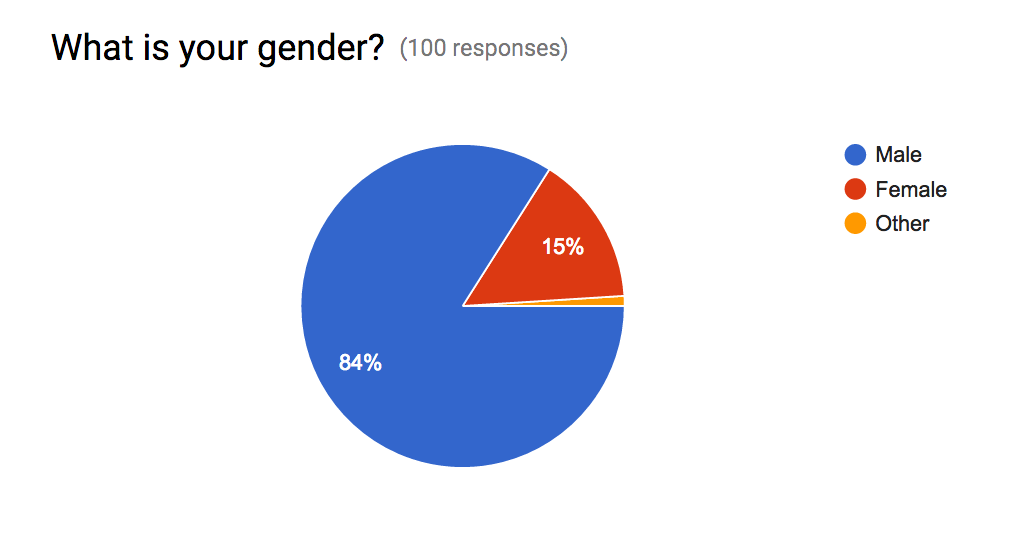
\includegraphics[width=1.0\textwidth]{sr-gender}
\caption{Gender distribution.}
\end{figure}
\item \textit{What is your gender?}
In Fall 2016, there was a total of 445 ICS students. Of the 445, 366 identified as male and 79 identified as female. This means that there was roughly 18\% females and 82\% males. The distribution of my survey has close proportions: 15\% female, 84\% male, and 1\% other. 
\begin{figure}[h]
\centering
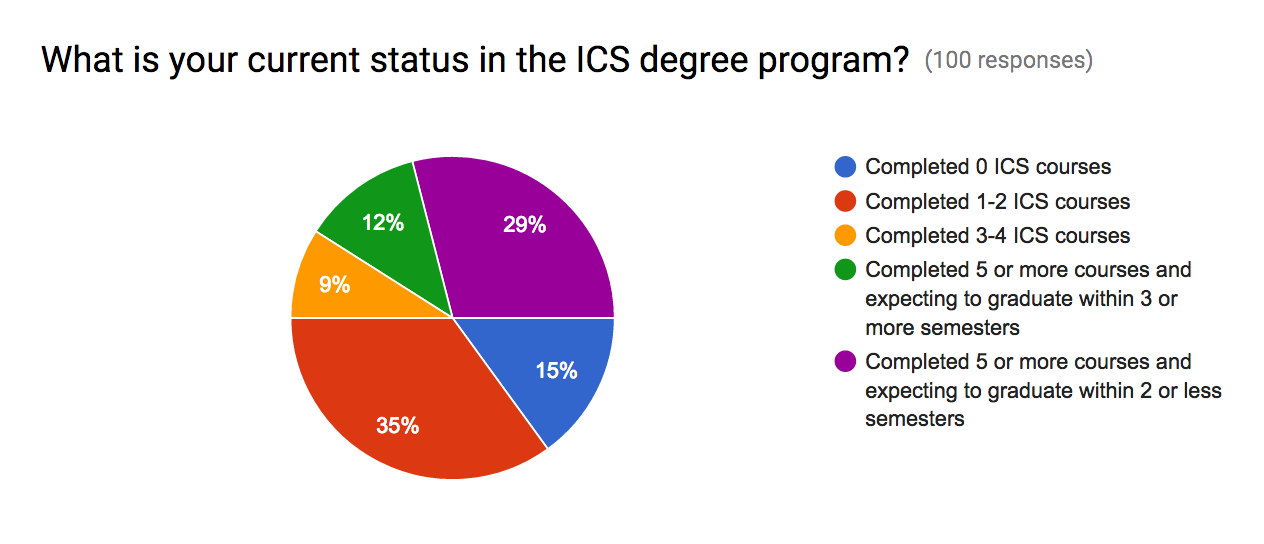
\includegraphics[width=1.0\textwidth]{sr-program-status}
\caption{ICS program status distribution.}
\end{figure}
\item \textit{What is your current status in the ICS degree program?}
The two most represented groups in the survey are those that had completed 1-2 ICS courses (35\%) and those that had completed 5 or more courses and expected to graduate within 3 or more semesters (29\%). 15\% of students surveyed were either in or about to start their first semester of ICS. Together, students who were in the middle of the program (completed 3-4 courses or 5 or more courses and expected to graduate within 3 or more semesters) comprised of 21\% of the total population surveyed. The fact that most of the students surveyed were either in the beginning of the program or about to graduate can be attributed to the fact that these are the students that physically go in for advising the most. 
\end{enumerate}

\section{Prospective ICS Students}
\begin{enumerate}
\begin{figure}[h]
\centering
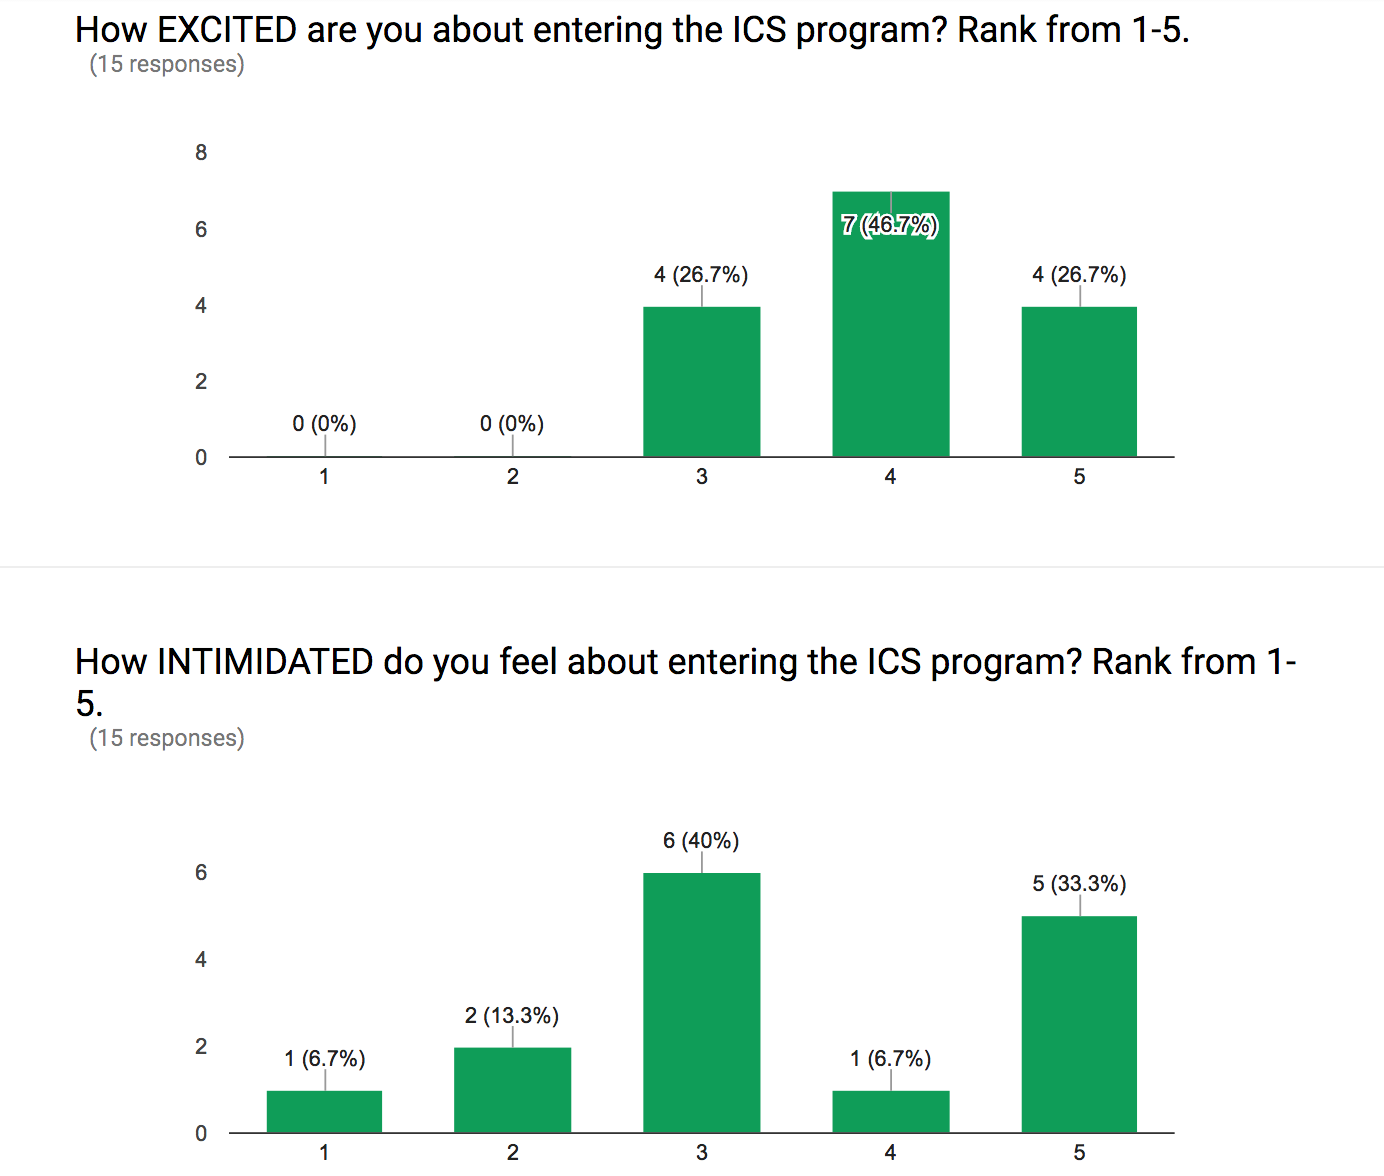
\includegraphics[width=1.0\textwidth]{sr-excited-intimidated}
\caption{Results for prospective ICS Students survey}
\end{figure}
\item\textit{How EXCITED are you about entering the ICS program? Rank from 1-5.}
The results of the survey show that all of the students surveyed felt either neutral or excited about entering the ICS program. No students stated that they were not excited. Further studies would be required to understand more behind the outside factors that affect incoming students' perceptions of the department. 
\item \textit{How INTIMIDATED do you feel about entering the ICS program? Rank from 1-5.}
The results of the survey show that a majority of the students surveyed (12 out of 15) felt either neutral or intimidated about entering the ICS program. None of the females surveyed felt less than neutral in regards to intimidation, while three males did feel less than neutral. Further studies would be required to understand more behind the outside factors that affect incoming students' feelings towards the department, and to understand if there are any differences in feelings between genders.
\end{enumerate}

\section{Current ICS Students}
\begin{enumerate}
\begin{figure}[h]
\centering
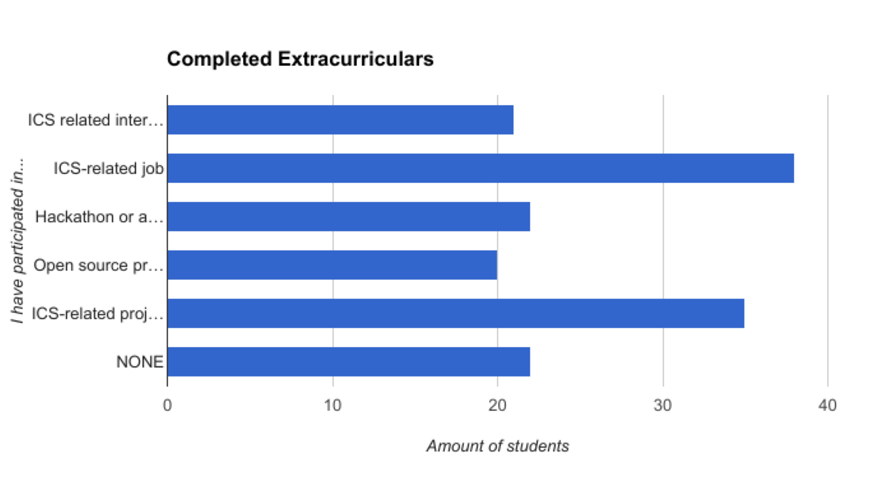
\includegraphics[width=1.0\textwidth]{sr-extracurric-bar}
\caption{Results for extracurricular participation by event type.}
\end{figure}

\begin{figure}[h]
\centering
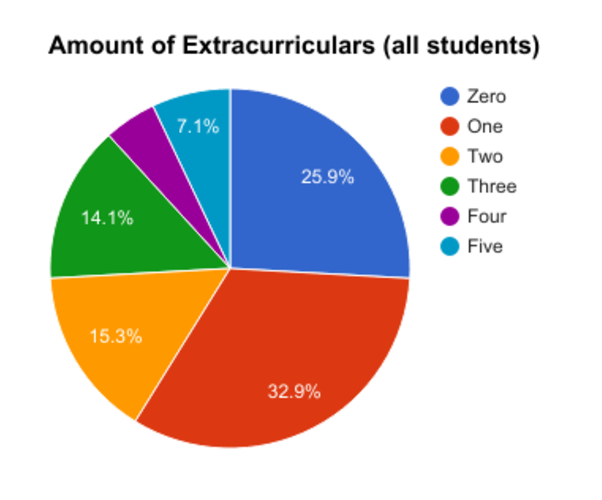
\includegraphics[width=1.0\textwidth]{sr-extracurric-pie}
\caption{Results for extracurricular participation by amount of participation (all students).}
\end{figure}

\begin{figure}[h]
\centering
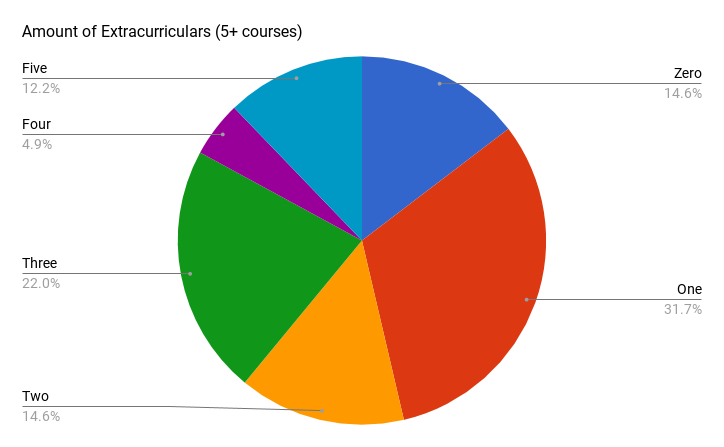
\includegraphics[width=1.0\textwidth]{sr-extracurric-pie-midgrad}
\caption{Results for extracurricular participation by amount of participation (mid to graduating students only).}
\end{figure}
\item \textit{Which of the following extracurricular activities, if any, pertain to you?}
Survey results show that out of all the extracurricular activities, the most common was having an ICS related job (38 students), with a close second being doing an ICS-related project outside of class (35 students)(Figure 5.4). Participating in an ICS-related internship, hackathon, or open source project each had about 20 students (21, 22, and 20, respectively). Another 22 students hadn't participated in any extracurricular activities. 

Another way to view this data is by the amount of extracurricular participation. In Figure 5.5, the results show the amount of extracurricular activities that each student participated in. A quarter of students (25.9\%) participated in zero extracurricular activities. About a third of students (32.9\%) participated in just one extracurricular activity. Overall, the amount of extracurricular activities is negatively correlated to the amount of students participating in them. 
To account for the fact that students in their first year of ICS are at a disadvantage when it comes to extracurricular participation (due to the lack of time and experience), Figure 5.6 looks at only those students who have completed at least 5 ICS courses. This graph shows that a majority of these students have participated in one extracurricular activity (40.6\%). 21.9\% of students have participated in two extracurricular activities, 15.6\% of students have participated in 0 extracurricular activities, 15.6\% of students have participated in five extracurricular activities, and 6.3\% of students have participated in four extracurricular activities. While this data shows higher levels of participation with mid to graduating students, there are still a significant amount of students who are not participating in any extracurricular activities or participating in only one or two. Ideally, RadGrad will increase both the amount and diversity of extra curricular activities that each student participates in.
\begin{figure}[h]
\centering
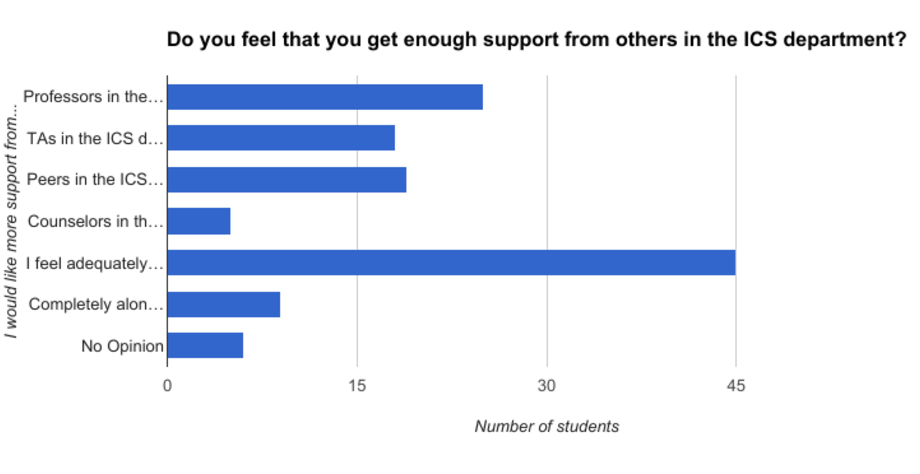
\includegraphics[width=1.0\textwidth]{sr-support-bar}
\caption{Results for support by types of support.}
\end{figure}

\begin{figure}[h]
\centering
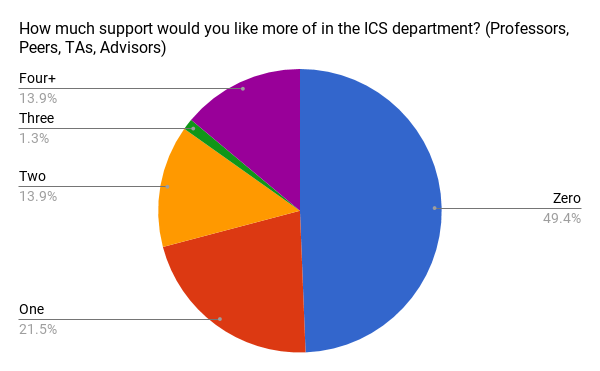
\includegraphics[width=1.0\textwidth]{sr-support-pie}
\caption{Results for support by amount of support desired}
\end{figure}
\item \textit{Do you feel that you get enough support from others in the ICS department?}
Survey results show that a majority of students (45 students) feel adequately supported in the ICS department (Figure 5.7). However, significant amounts of students desire more support in various areas. 25 students desire more support from professors, 19 students desire more support from their peers, 18 students desire more support from TAs, and 5 students desire more support from advisors. Additionally, 9 students stated that they often feel completely alone in the ICS department and only depend on themselves. 

Another way to view this data is by the extent of the support requested. In Figure 5.8, the results show the amount of support requested by each student. This graph shows that almost half of the students did not request any further support (49.4\%), while the other half requested further support from at least one group. 21.5\% of students requested further support from one group, 13.9\% requested further support from two groups, 13.9\% requested further support from four or more groups, and 1.3\% requested further support from three groups. Further studies could gather more information about exactly how students would like support to be given, and ideally after RadGrad, a majority of students will feel adequately supported, and less students will feel completely alone within the department. 
\begin{figure}[h]
\centering
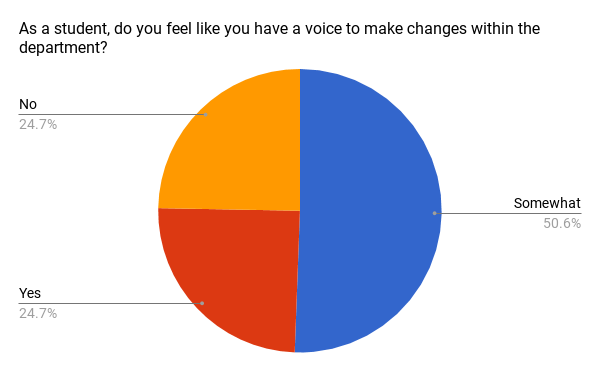
\includegraphics[width=1.0\textwidth]{sr-changes}
\caption{Results for feelings about having a voice to make changes.}
\end{figure}
\item \textit{As a student, do you feel like you have a voice to make changes within the department?}
Results show that only a quarter of the students surveyed (24.7\%) definitely felt like they have a voice to make changes within the department (Figure 5.9). Another quarter (24.7\%) feel like they definitely do not have a voice to make changes, while about half (50.6\%) only somewhat feel like they have a voice to make changes. While the current version of RadGrad does not directly address this issue, it may be addressed in future expansions on RadGrad, such as with the petition feature. In the future, further studies should be conducted to test whether RadGrad has an affect on whether students feel like they have a voice or not. Ideally, after RadGrad, more than 25\% of the students will feel like they definitely have a voice to make changes within the department.
\begin{figure}[h]
\centering
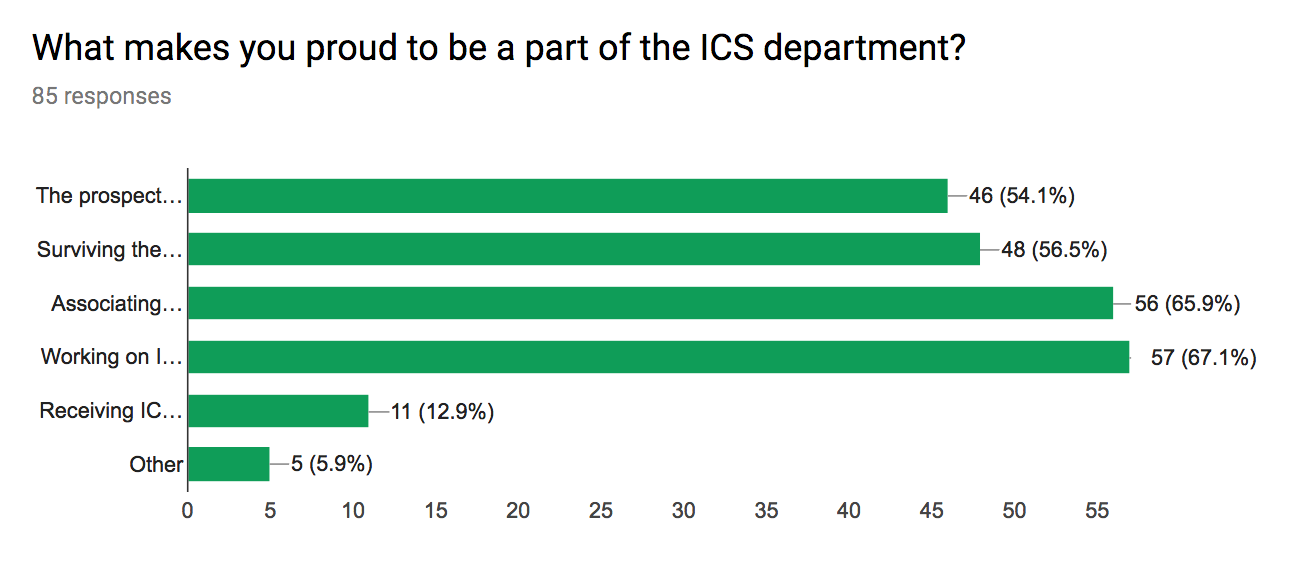
\includegraphics[width=1.0\textwidth]{sr-proud}
\caption{Results for reasons for being proud to be a part of the ICS department.}
\end{figure}
\item \textit{What makes you proud to be a part of the ICS department?}
Survey results show that a majority of students had at least one reason to feel proud to be a part of the ICS department. The most popular reasons (in order of decreasing popularity) were working on ICS related projects, associating with the people in ICS, surviving the rigorousness of ICS, and the prospect of finding a high paying job after graduation. The least popular reason, with only 11 students, was receiving ICS awards. Another 5 students chose ``other" without giving a specific reason. Future studies can be held to see whether or not RadGrad increases the amount of pride within the ICS community. By enhancing the ICS experience overall, RadGrad will hopefully encourage students to view the department in a more positive way. 
\end{enumerate}

\section{Current ICS Students: Influences}
\begin{enumerate}
\begin{figure}[h]
\centering
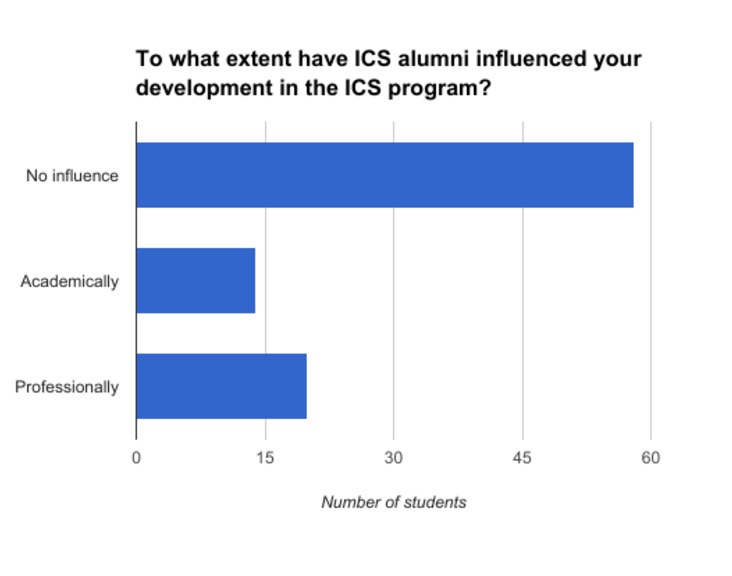
\includegraphics[width=1.0\textwidth]{sr-alumni-influence}
\caption{Results for alumni influence}
\end{figure}
\item \textit{To what extent have ICS alumni influenced your development in the ICS program?}
Survey results show that a majority of students (58 our of 84 students) have not been influenced by alumni in any professional or academic way, while 20 out of 84 students have been influenced by an alumni to improve professional development, and 14 out of 84 students have been influenced by an alumni to pursue a major in ICS (Figure 5.11). This suggests that many current ICS students are not interacting with ICS alumni. Further studies should test to see if RadGrad adequately provides a way for more students to easily interact with and become influenced by alumni. In the future, this question could be changed to more broad in terms of academic and professional influence. Ideally, after RadGrad, a majority of students will have been influenced by alumni in either an academic or professional way.   
\begin{figure}[h]
\centering
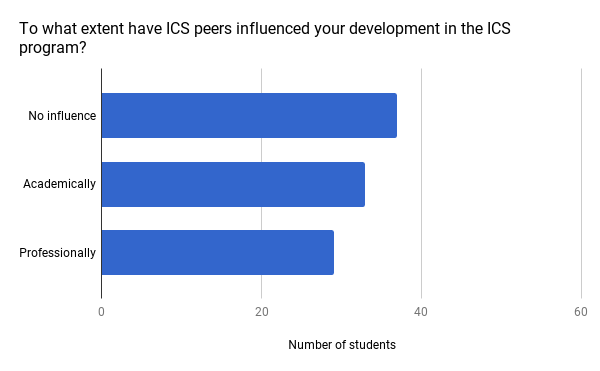
\includegraphics[width=1.0\textwidth]{sr-peer-influence}
\caption{Results for peer influence}
\end{figure}
\item \textit{To what extent have ICS peers influenced your development in the ICS program?}
Survey results show that a little less than half of students (37 out of 85 students) have not been influenced by their peers in any professional or academic way, while 33 out of 85 students have been influenced by a peer to pursue a major in ICS, and 29 out of 85 students have been influenced by a peer to improve professional development (Figure 5.12). This suggests that there is room for improvement when it comes to encouraging academic and professional collaboration among peers. Further studies should test to see if RadGrad adequately provides a way for more students to easily interact with and become influenced by each other. In the future, this question could be changed to more broad in terms of academic and professional influence. Ideally, after RadGrad, at least 75\% of students will have been influenced by a peer in either an academic or professional way. 
\begin{figure}[h]
\centering
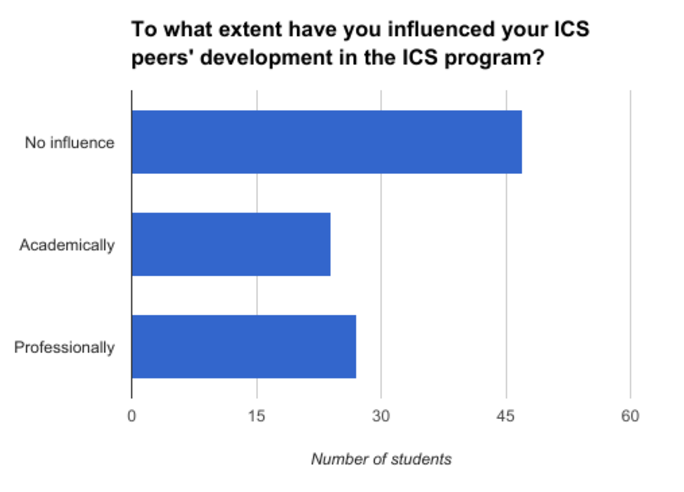
\includegraphics[width=1.0\textwidth]{sr-self-influence}
\caption{Results for student perceptions of their own influence}
\end{figure}
\item \textit{To what extent have you influenced your ICS peers’ development in the ICS program?}
Survey results show that over half of students (49 out of 85 students) feel like they have not influenced their peers in any professional or academic way, while 27 out of 85 students feel like they have influenced a peer to improve professional development, and 25 out of 85 students feel like they have influenced a peer to pursue a major in ICS (Figure 5.13). This suggests that there is room for improvement when it comes to encouraging academic and professional collaboration among peers. Further studies should test to see if RadGrad adequately provides a way for more students to easily interact with and influence their peers. In the future, this question could be changed to more broad in terms of academic and professional influence. Ideally, after RadGrad, a majority of students will feel like they have influenced a peer in either an academic or professional way. 
\end{enumerate}

\section{Graduating ICS Students}
\begin{enumerate}
\begin{figure}[h]
\centering
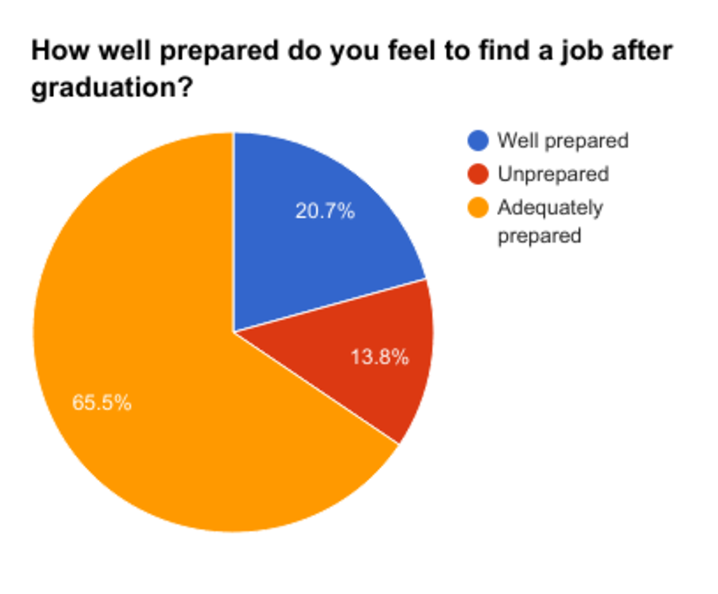
\includegraphics[width=1.0\textwidth]{sr-prepared}
\caption{Results for graduation preparedness.}
\end{figure}
\item \textit{Now that you are nearing the end of your ICS degree program experience, how well prepared do you feel to find a job after graduation?}
Survey results show that only 20.7\% of graduating students feel well prepared to find a job after graduation (Figure 5.14). 65.6\% of graduating students feel adequately prepared, and 13.8\% of students feel unprepared. This suggests that there is room for improvement when it comes to preparing students for the workforce in a way that makes them feel confident and prepared. Further studies should test to see if RadGrad's encouragement of collaboration and a well-balanced education (with both courses and opportunities) causes more students to feel well prepared to find a job after graduation. Ideally, after RadGrad, a majority of students will feel like they are well prepared to find a job after graduation. 
\begin{figure}[h]
\centering
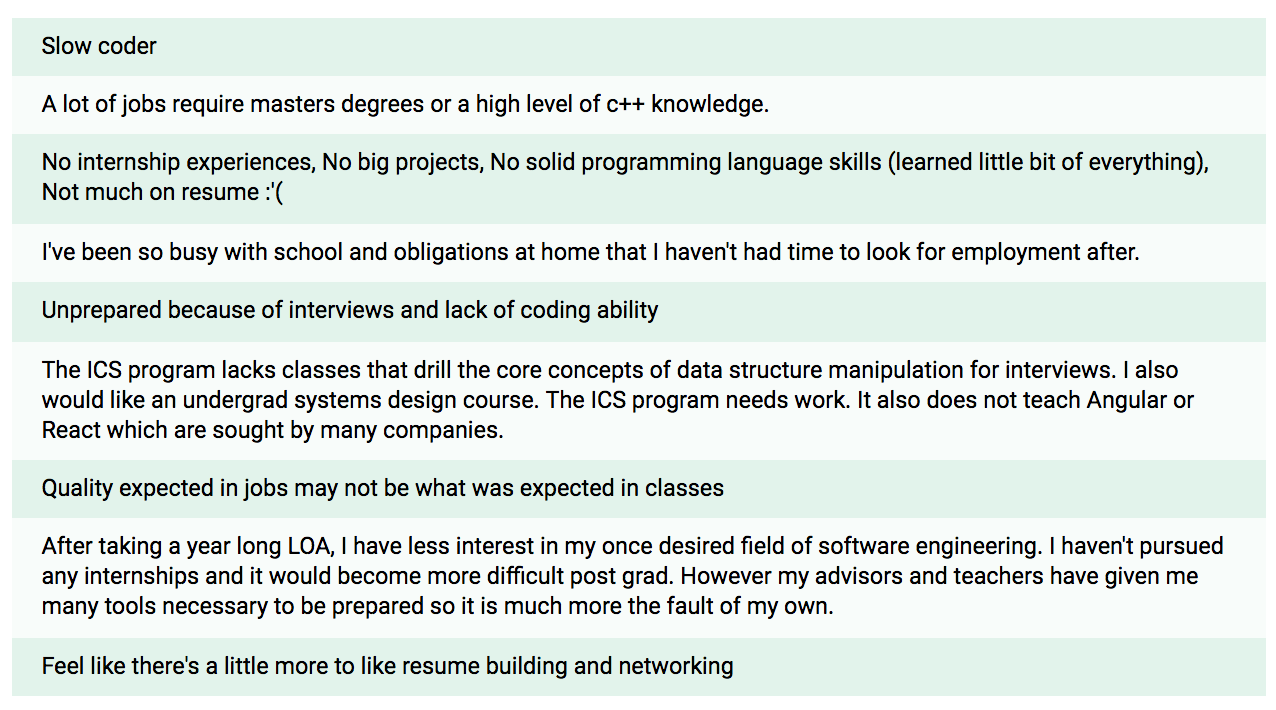
\includegraphics[width=1.0\textwidth]{sr-unprepared-grad-reasons}
\caption{Reasons for not feeling prepared for graduation.}
\end{figure}
\item \textit{If you answered above that you feel unprepared to find a job after graduation, please explain why. }
Figure 5.15 lists reasons that students have for not feeling well prepared to find a job after graduation. These reasons suggest that RadGrad could have a positive impact by encouraging students to pursue ICS related experiences outside of the classroom. Ideally, after RadGrad, the reasons given for not feeling well prepared will not focus on the lack of outside experience. 
\end{enumerate}


